
This section describes an application of ElecSIM. Here, we vary the carbon tax and either grow or reduce total electricity demand. This was done to observe the effects of carbon tax policy on long-term investment.

We assume that carbon tax is set by the government, and not subject to market forces such as the EU Emissions Trading Scheme \cite{Council2016}.



%\begin{figure}[h]
%	\begin{center}
%		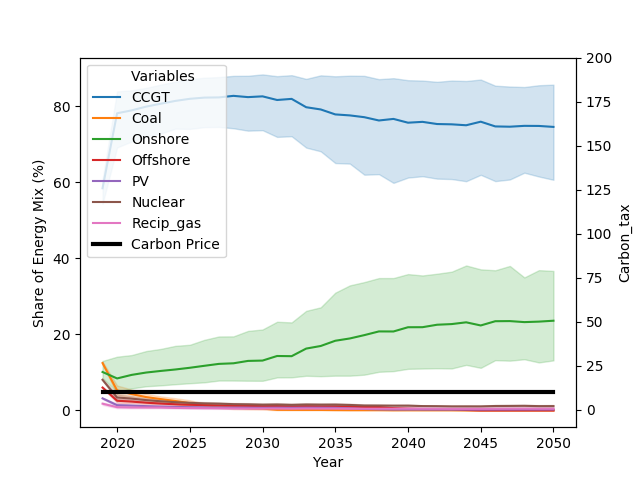
\includegraphics[width=0.5\textwidth]{figures/scenarios/demand099-carbon10-datetime.png}
%		\caption{Demand decreasing by 1\% per year and a carbon tax of \textsterling10}
%		\label{fig:demand99carbon10}
%	\end{center}
%\end{figure}
%
%\begin{figure}[h]
%	\begin{center}
%		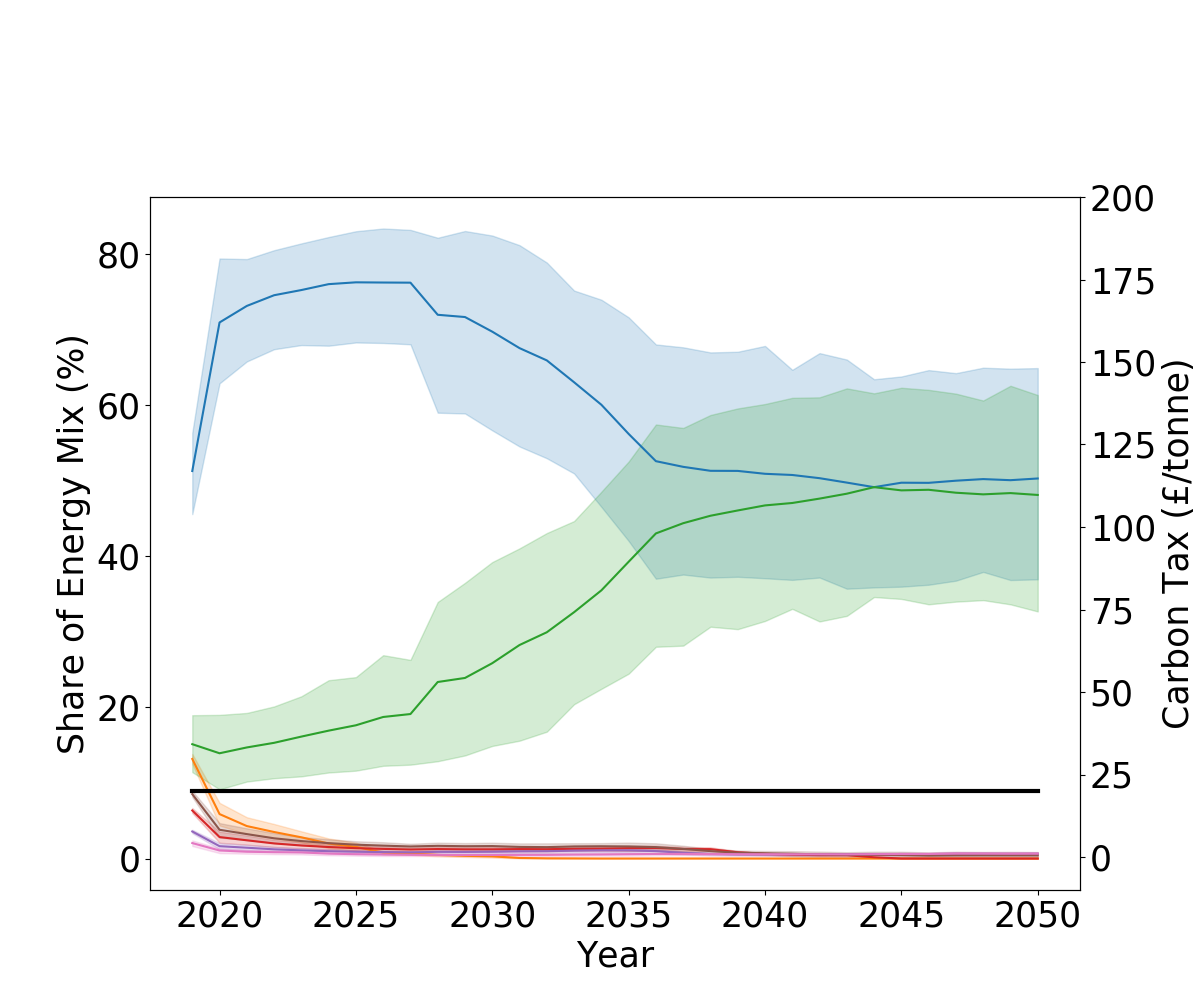
\includegraphics[width=0.5\textwidth]{figures/scenarios/demand099-carbon20-datetime.png}
%		\caption{Demand decreasing by 1\% per year and a carbon tax of \textsterling20}
%		\label{fig:demand99carbon10}
%	\end{center}
%\end{figure}
%
%
%
%\begin{figure}[h]
%	\begin{center}
%		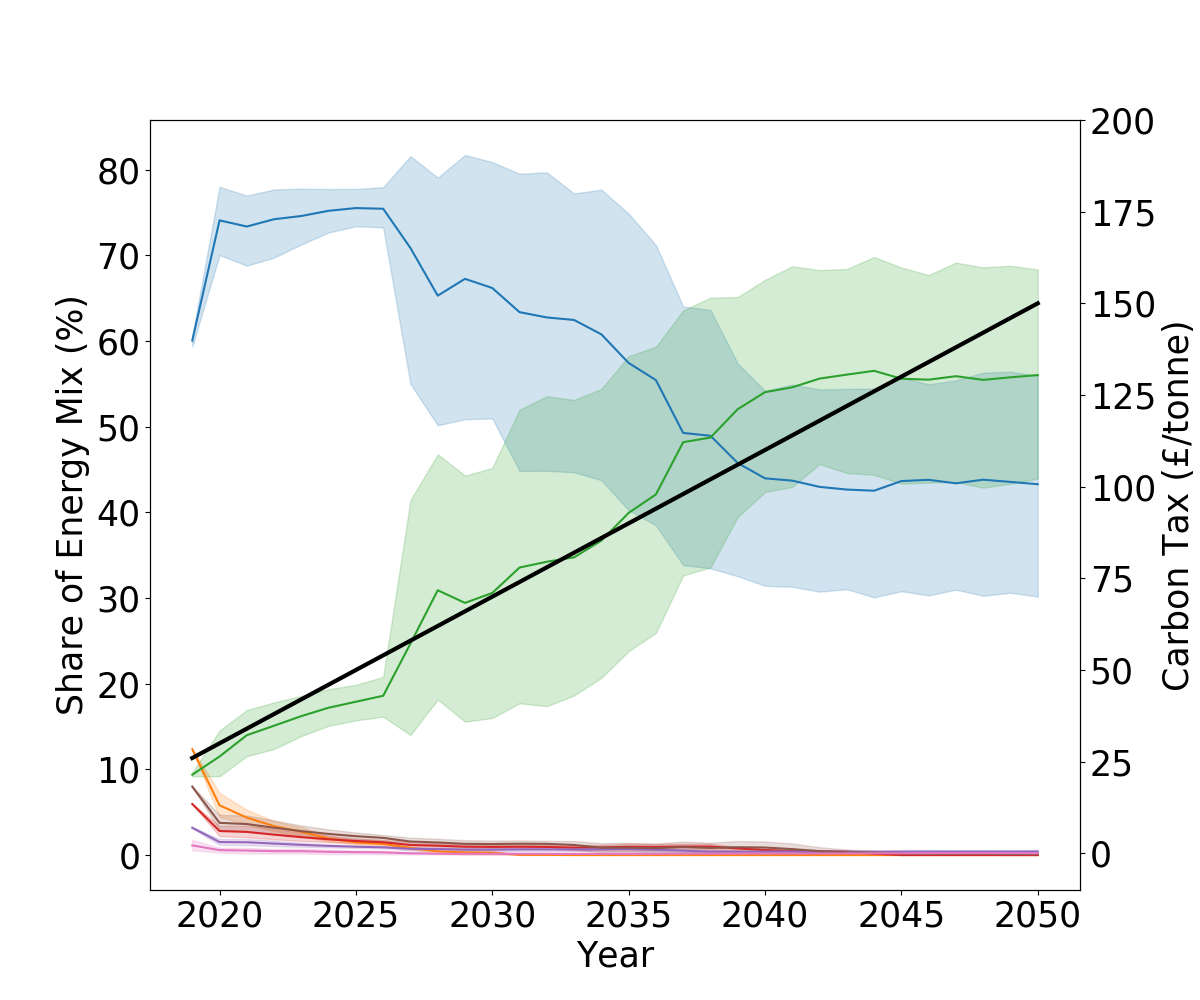
\includegraphics[width=0.5\textwidth]{figures/scenarios/demand099-carbon18-datetime.png}
%		\caption{Demand decreasing by 1\% per year and a carbon tax of \textsterling20}
%		\label{fig:demand99carbon10}
%	\end{center}
%\end{figure}
%
%
%
%\begin{figure}[h]
%	\begin{center}
%		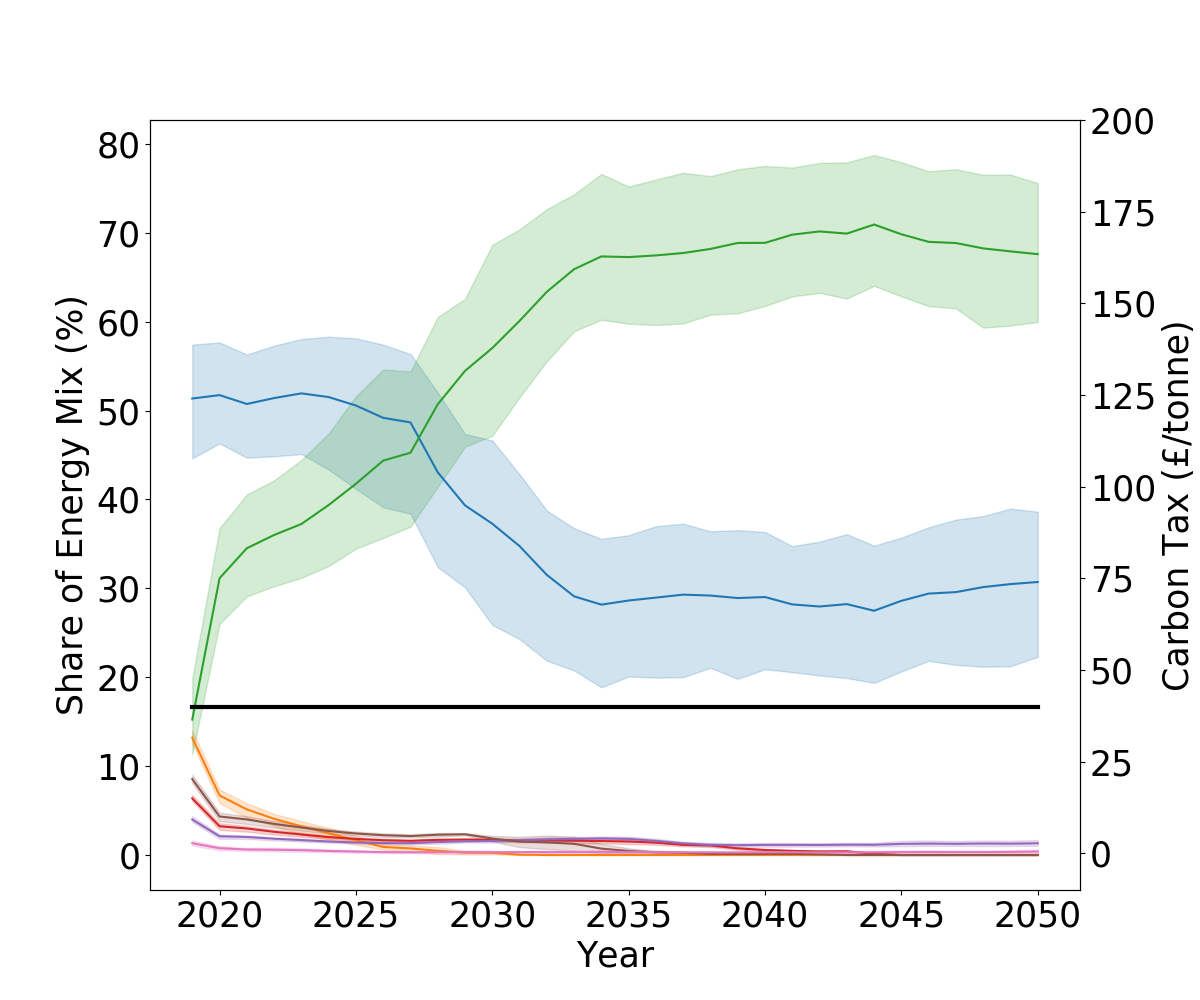
\includegraphics[width=0.5\textwidth]{figures/scenarios/demand099-carbon40-datetime.png}
%		\caption{Demand decreasing by 1\% per year and a carbon tax of \textsterling20}
%		\label{fig:demand99carbon10}
%	\end{center}
%\end{figure}










\begin{figure*}[h!]
	\centering
	\begin{subfigure}[b]{0.475\textwidth}
		\centering
		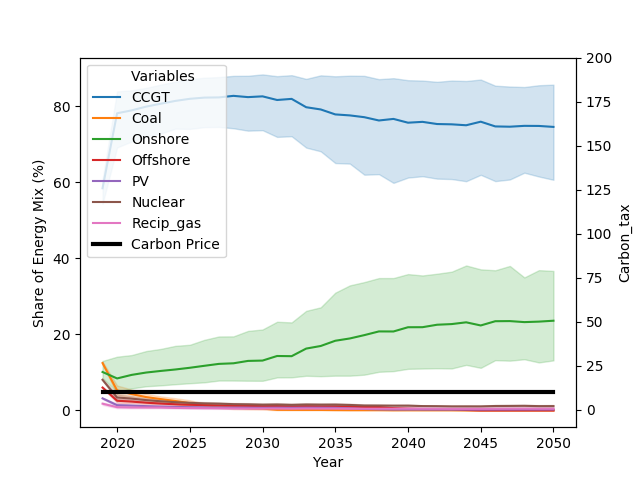
\includegraphics[width=\textwidth]{figures/scenarios/demand099-carbon10-datetime.png}
		\caption[Network2]%
		{{\small \textsterling10 carbon tax}}    
		\label{fig:demand99carbon10}
	\end{subfigure}
	\hfill
	\begin{subfigure}[b]{0.475\textwidth}  
		\centering 
		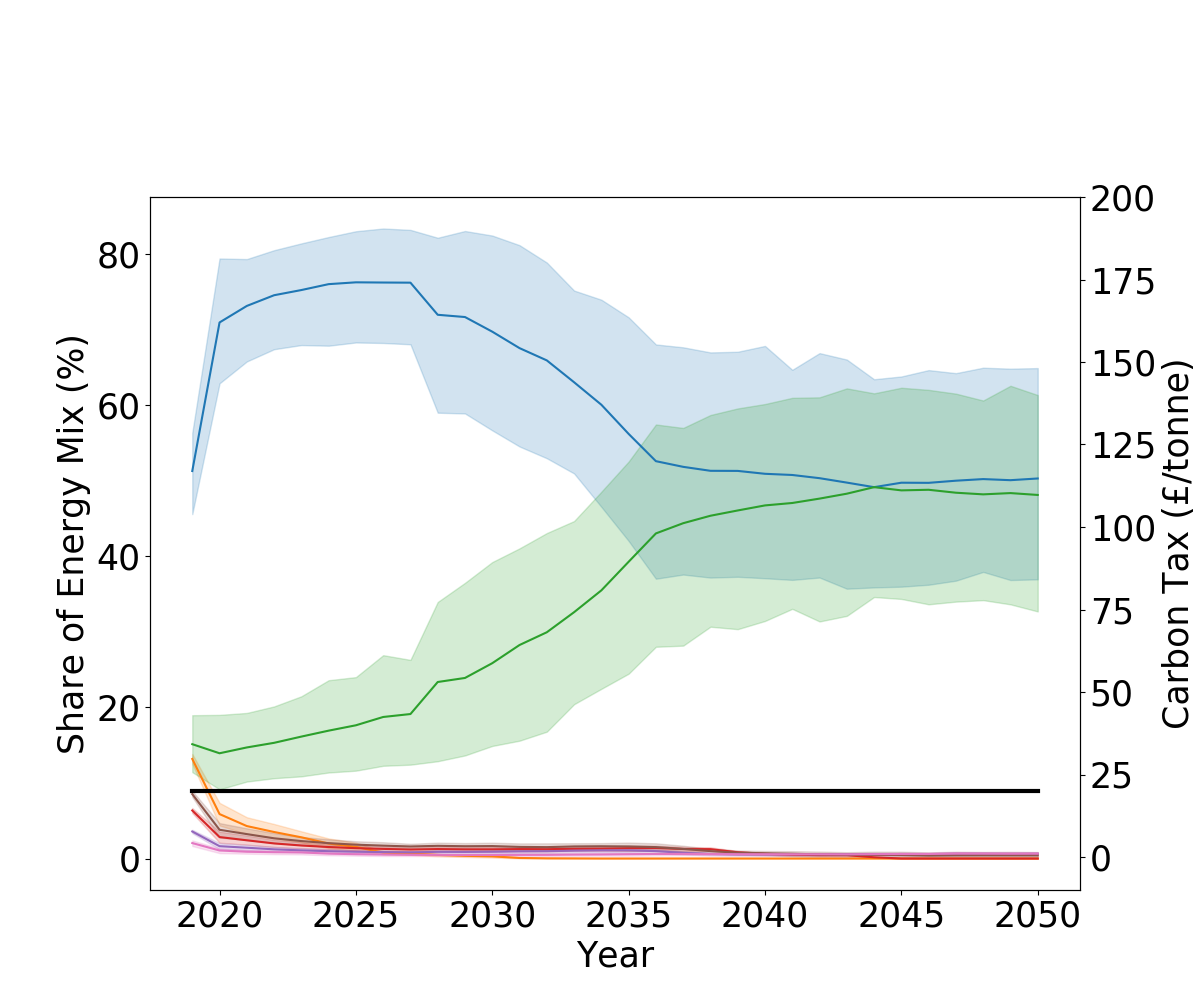
\includegraphics[width=\textwidth]{figures/scenarios/demand099-carbon20-datetime.png}
		\caption[]%
		{{\textsterling20 carbon tax}}    
		\label{fig:demand99carbon20}
	\end{subfigure}
	\vskip\baselineskip
	\begin{subfigure}[b]{0.475\textwidth}   
		\centering 
		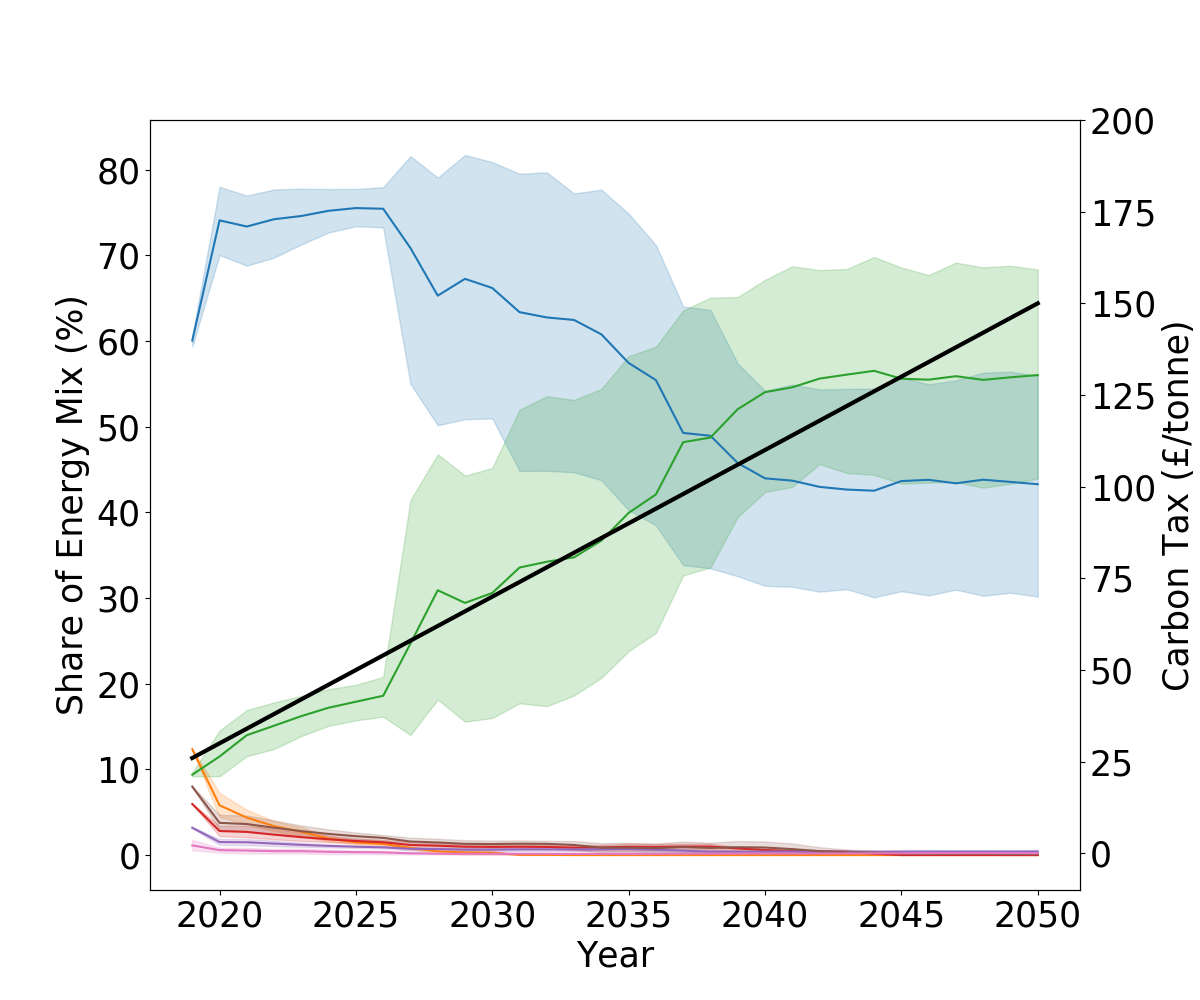
\includegraphics[width=\textwidth]{figures/scenarios/demand099-carbon18-datetime.png}
		\caption[]%
		{{\textsterling18 to \textsterling178 linearly increasing carbon tax}}    
		\label{fig:demand99carbon18}
	\end{subfigure}
	\quad
	\begin{subfigure}[b]{0.475\textwidth}   
		\centering 
		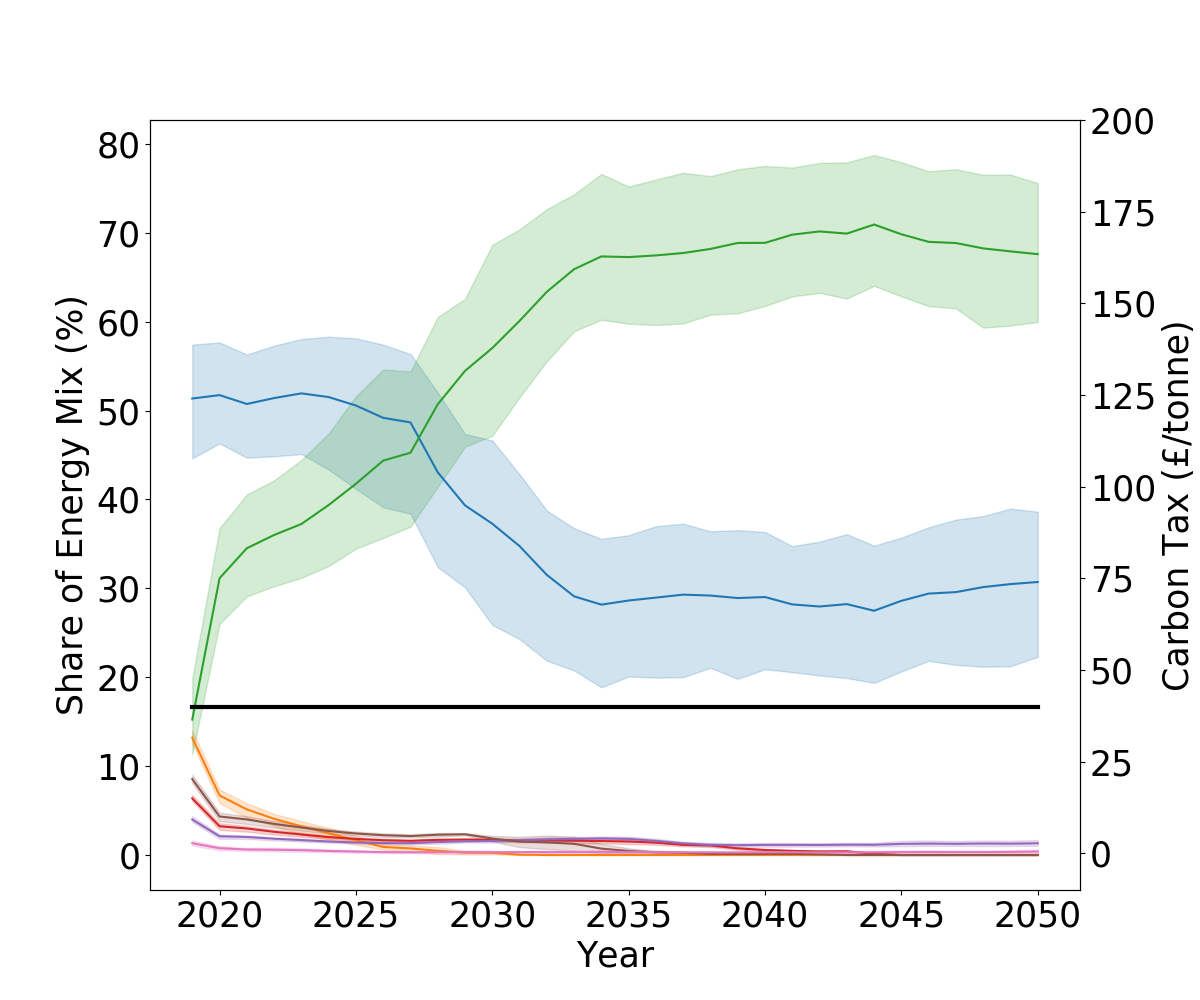
\includegraphics[width=\textwidth]{figures/scenarios/demand099-carbon40-datetime.png}
		\caption[]%
		{{\textsterling40 carbon tax}}    
		\label{fig:demand99carbon40}
	\end{subfigure}
	\caption[ Scenarios up to the year 2050 with varying carbon taxes and decreasing demand ]
	{\small Scenarios up to the year 2050, with varying carbon taxes and decreasing electricity demand} 
	\label{fig:mean and std of nets}
\end{figure*}



\begin{itemize}
	\item Effect of different carbon tax on investments made.
	\item Effects of different demand scenarios. (High peaks, high growth, high reduction in demand)
	\item Effects of high fuel prices.
	\item Different costs of capital (eg. Borrowing for Nuclear of interest rate to equal 2\% at government bonds rate, as opposed to 10\% for private companies.)
	\item Different learning rates for renewable costs.
	\item The effect of long term carbon tax policy (eg. Carbon price known for next 25 years) vs short term changes in carbon tax.
\end{itemize}
